\def\GraphicsFolder{parts/mft-analysis/chapters/mft-discussion/pictures}
\chapter{Mean-field theory discussion of the EHM}\label{chap:mft-discussion}

This chapter is devoted to develop a Mean Field Theory (MFT) framework of the Extended Hubbard model (EHM) of Eq.~\eqref{eq:extended-hubbard-model},
\[
	\hat H =
	\underbrace{
		-t \sum_{\langle ij \rangle} \sum_\sigma \hat c_{i\sigma}^\dagger \hat c_{j\sigma}
	}_{\hat H_t} \underbrace{
		+U \sum_i \hat n_{i\uparrow} \hat n_{i\downarrow}
		\vphantom{
			\sum_{\langle ij \rangle}
		}
	}_{\hat H_U}
	\underbrace{
		- V \sum_{\langle ij \rangle} \sum_{\sigma \sigma'} \hat n_{i\sigma} \hat n_{j\sigma'}
	}_{\hat H_V}
\]
Mean Field Theory (MFT) is a widely used and simple theoretical tool, often sufficient to describe the leading orders in phase transition phenomena of Many-Body Physics. Here MFT is employed generically, in order to later discuss both the effects of the non-local term $\hat H_V$ onto the AF phase (Chap.~\ref{chap:mft-af-instability}), as well as the insurgence of anisotropic superconductivity (Chap.~\ref{chap:mft-su-instability}). The latter, following the path of Bardeen-Cooper-Schrieffer (BCS) theory in describing conventional $s$-wave superconductivity. As will be thoroughly described, the lattice spatial structure directly influences the topology of the gap function, giving rise to anisotropic pairing.

{
	\color{tabred}[ Move this part to Chap.~\ref{chap:mft-su-instability} ]
	Sec.~\ref{sec:mft-analysis-non-local-source} studies the non-local attraction $\hat H_V$ in real-space, describing how such interaction can contribute to the hamiltonian as a symmetry-breaking term in given channels. In the following sections, we move to specific channels and study theoretically and numerically the effect of non-local attraction.
}

\section{Extended Hubbard model symmetries and Wick's theorem}\label{sec:ehm-symmetries}

The general aim is to study the phase diagram of the model by comparing ground-state energies of different phases. The phases we consider in next chapters for the EHM are the Anti-Ferromagnetic ordering (AF), given by a non-uniform distribution of charge in each spin sector, and the Superconducting phase, described by a uniformly distributed charge allowing for Cooper pairing instabilities. The first evident symmetry of the model is a global $\mathrm{U}(2)$ symmetry \cite{arovas2022hubbard} given by the transformation
\begin{equation}\label{eq:ehm-global-u2-symmetry}
	\hat c_{i\sigma} \to \sum_{\sigma'} \mathcal{U}_{\sigma \sigma'} \hat c_{i\sigma'}
	\qq{with}
	\mathcal{U}_{\sigma \sigma'} \in \mathrm{U}(2)
\end{equation}
The proof is trivial and follows from the fact that $\mathcal{U}^\dagger \mathcal{U} = \mathcal{U} \mathcal{U}^\dagger = \Id$. Note that the the following decomposition holds,
\begin{equation}\label{eq:ehm-global-u2-symmetry-u1-su2}
	\mathrm{U}(2) = \mathrm{SU}(2) \otimes \mathrm{U}(1)
\end{equation}
which expresses the separate charge conservation and spin rotational symmetries. Thus, for the EHM, three symmetries are ``brekable'':
\begin{enumerate}
	\item Discrete translational invariance. By breaking explicitly this symmetry, the obtained state must show a Charge-Density Wave (CDW) ordering;
	\item $\mathrm{U}^\mathrm{c}(1)$ charge conservation, coming from Eq.~\eqref{eq:ehm-global-u2-symmetry-u1-su2} decomposition. By breaking this symmetry, we allow for the total charge to fluctuate in the ground state;
	\item $\mathrm{SU}(2)$ spin rotation symmetry, also , coming from Eq.~\eqref{eq:ehm-global-u2-symmetry-u1-su2} decomposition. If this symmetry is broken, we allow for the ground state to exhibit a preferred spin direction.
	\item Note that the $\mathrm{SU}(2)$ group contains itself a $\mathrm{U}(1)$ subgroup. $\mathrm{SU}(2)$ symmetry can be broken, selecting a particular vectorial direction for the order parameter, and reduced to a smaller $\mathrm{U}^z(1)$ symmetry which is essentially expressed by the conservation of the \textit{magnitude} of the order parameter.
\end{enumerate}
The last point is important: for the AF phase, for example, there is no need for the magnetization vector to be directed along the \textit{real} $z$-axis, which is the one perpendicular to the lattice plane. $\mathrm{SU}(2)$ symmetry breaks when (staggered) magnetization is established along a particular direction, but spin rotations around said direction still are ground state symmetries. The symmetries are reported synthetically in Tab.~\ref{tab:symmetry-groups}.

\begin{figure}
	\centering
	\subfloat[$\mathrm{SU}(2)$ rotations domain before SSB.]{
		\def\rotationSphere{-100}
\def\tiltsphere{20}
\def\radiusSphere{2cm}
\begin{blochsphere}[
	radius=\radiusSphere,
	tilt=\tiltsphere,
	rotation=\rotationSphere,
	opacity=0.1,
	color=tabblue
	]
	% --- Ball setup ---
	\drawBallGrid[style={opacity=0.05}]{30}{45}
	\drawLongitudeCircle[style={dashed,color=lightgray}]{0}
		\drawLongitudeCircle[style={dashed,color=lightgray}]{90}
	\drawLatitudeCircle[style={dashed,color=lightgray}]{0}
	
	% --- Points ---
	\labelLatLon{z+}{90}{0};
	\labelLatLon{z-}{-90}{0};
	\labelLatLon{x-}{0}{180};
	\labelLatLon{x+}{0}{0};
	\labelLatLon{y+}{0}{270};
	
	% --- Axis ---
	\draw[-stealth]
		(0,0) -- ($($(0,0)!0.5!(z+)$)$) node[anchor=south] {\footnotesize $z$};
	\draw[-stealth] 
		(0,0) -- ($($(0,0)!0.5!(x+)$)$) node[anchor=east,yshift=-0.2em] {\footnotesize$x$};
	\draw[-stealth] 
		(0,0) -- ($($(0,0)!0.5!(y+)$)$) node[anchor=west,yshift=-0.1em] {\footnotesize $y$};
			
\end{blochsphere}
		\label{subfig:su2-domain}	
	}
	\hspace{2em}
	\subfloat[$\mathrm{U}(1)$ rotations domain after SSB.]{
		\def\rotationSphere{-100}
\def\tiltsphere{25}
\def\ThetaParameter{45}
\def\PhiParameter{80}
\def\radiusSphere{2cm}
\begin{blochsphere}[
	radius=\radiusSphere,
	tilt=\tiltsphere,
	rotation=\rotationSphere,
	opacity=0
	]
	% --- Ball setup ---
	\drawBallGrid[style={opacity=0.05}]{30}{45}
	
	% --- Points ---
	\labelLatLon{z+}{90}{0};
	\labelLatLon{z-}{-90}{0};
	\labelLatLon{x-}{0}{180};
	\labelLatLon{x+}{0}{0};
	\labelLatLon{y+}{0}{270};
	\labelLatLon{versor}{\ThetaParameter}{-\PhiParameter};
	
	% Rotation
	\drawGreatCircle[style={dashed,color=tabblue}]{\ThetaParameter}{-\PhiParameter}
	\drawRotationRight[scale=1.1,style={color=tabblue}]{\ThetaParameter}{-\PhiParameter}{0}{15}	
	
	% --- Axis ---
	\draw[-stealth,color=lightgray]
		(0,0) -- ($($(0,0)!0.5!(z+)$)$) node[anchor=south] 
			{\footnotesize $z$};
	\draw[-stealth,color=lightgray] 
		(0,0) -- ($($(0,0)!0.5!(x+)$)$) node[anchor=east,yshift=-0.2em] 
			{\footnotesize$x$};
	\draw[-stealth,color=lightgray] 
		(0,0) -- ($($(0,0)!0.5!(y+)$)$) node[anchor=west,yshift=-0.1em] 
			{\footnotesize $y$};
	
	% --- Versor ---
	\draw[color=tabblue,-stealth]
		(0,0) -- (versor) node[anchor=south west]
			{$\mathbf{m}$};
\end{blochsphere}
		\label{subfig:u1-domain}
	}
	\caption{Graphic representation of the concept of $\mathrm{SU}(2)\to\mathrm{U}(1)$ SSB. The blue color identifies, in both cases, the rotations domain for the current symmetry. When SSB takes place in a magnetic phase, the magnetization order parameter acquires a precise direction which was previously invariant over the full spherical domain. After SSB, the hamiltonian is rotationally invariant only for rotations \textit{around} the selected magnetization vector.}
	\label{fig:su2-u1-domains}
\end{figure}

\begin{table}
	\centering
	\begin{tabular}{c l}
		\textbf{Symmetry group} & \textbf{Operations} \\
		\midrule
		Point group & Discrete translations on lattice \\
		$\mathrm{U}^\mathrm{c}(1)$ & Charge-conserving global phase shifts \\
		$\mathrm{SU}(2)$ & Three-dimensional rotations in spin space \\
		$\mathrm{U}^z(1)$ & Reduced two-dimensional rotations around order parameter after SSB \\
		\midrule
	\end{tabular}
	\caption{Model symmetries and relative group operations. Note that $U^\mathrm{c}(1)$ represents the charge conserving group, while $\mathrm{U}^z(1)$ represents the subgroup obtained by breaking the $\mathrm{SU}(2)$ symmetry with a vector order parameter and preserving its amplitude.}
	\label{tab:symmetry-groups}
\end{table}

Different phases are described by different order parameters, each one exhibiting a specific symmetry subset from the initial set, while the rest are broken. Ferromagnetic state perform $\mathrm{SU}(2) \to \mathrm{U}^z(1)$ spontaneous symmetry breaking (SSB), through the magnetic order parameter acquiring a specific spatial direction. Such SSB process is graphically depicted in Fig.~\ref{fig:su2-u1-domains}. Anti-ferromagnetic ordering breaks also translational invariance (reducing it to a smaller symmetry, relative to double-sized unitary cells). Basic superconducting models do not break translational invariance and can preserve full $\mathrm{SU}(2)$ symmetry, while breaking $\mathrm{U}^\mathrm{c}(1)$ charge conservation. The three phases hereby considered do not completely break translational invariance: the latter either is left untouched or is reduced to a weaker translational invariance. Because of this, it will be rather useful to move the framework to reciprocal space. We will get there in Sec.~\ref{subsec:mft-discussion-reciprocal-non-local}.

App.~\ref{appendix:mean-field-hubbard} describes in detail the MFT treatment of the pure Hubbard model, $\hat H_t + \hat H_U$ and its AF phase; the key passage is there given by the approximation
\begin{equation}\label{eq:mft-pure-hubbard-wick-decomposition}
	\hat n_{i\uparrow} \hat n_{i\downarrow} \simeq \hat n_{i\uparrow} \langle \hat n_{i\downarrow} \rangle + \langle \hat n_{i\uparrow} \rangle \hat n_{i\downarrow} + (\mathrm{constants})
\end{equation}
from which the AF structure is simply recovered. However, to perform the above approximation coherently, we are implementing Wick's Theorem on the generic term:
\begin{equation}\label{eq:mft-extended-hubbard-wick-decomposition}
	\langle
	\hat c_{i\sigma}^\dagger \hat c_{j\sigma'}^\dagger \hat c_{j\sigma'} \hat c_{i\sigma}
	\rangle \simeq \underbrace{
		\langle 
		\hat c_{i\sigma}^\dagger \hat c_{j\sigma'}^\dagger
		\rangle \langle	
		\hat c_{j\sigma'} \hat c_{i\sigma} 
		\rangle 
	}_{\text{Cooper}}
	- 
	\underbrace{
		\langle 
		\hat c_{i\sigma}^\dagger \hat c_{j\sigma'}
		\rangle \langle	
		\hat c_{j\sigma'}^\dagger \hat c_{i\sigma} 
		\rangle 
	}_{\text{Fock}}
	+ 
	\underbrace{
		\langle 
		\hat c_{i\sigma}^\dagger \hat c_{i\sigma}
		\rangle \langle	
		\hat c_{j\sigma'}^\dagger \hat c_{j\sigma'} 
		\rangle
	}_{\text{Hartree}}
\end{equation}
As a first approximation, the theorem is assumed to hold (which, in a $\mathrm{BCS}$-like fashion, is equivalent to assuming for the ground-state to be a coherent state). The AF ground state breaks translational invariance and reduces rotational symmetry, $\mathrm{SU}(2) \to \mathrm{U}^z(1)$. Thus, of the three terms above, when considering the pure Hubbard model: 
\begin{itemize}
	\item Cooper fluctuations are suppressed, because they break charge conservation;
	\item Similarly the Fock term is null as well because if $i=j$ and $\sigma'=\overline{\sigma}$ (as is for the local interaction, which contains the operator $\hat n_{i\uparrow} \hat n_{i\downarrow}$) the expectation values involved are describing a process breaking the survivor $\mathrm{U}^z(1)$ spin symmetry. 
\end{itemize}
Thus, correctly, the Wick's decomposition of Eq.~\eqref{eq:mft-pure-hubbard-wick-decomposition} only involves Hartree-terms of Eq.~\eqref{eq:mft-extended-hubbard-wick-decomposition}. In general, however, the three terms need to be considered altogether: this is what is done in the next chapters. 

\subsection{Particle-hole symmetry}

\todo For now, let us focus on the non-local term showing how can it break symmetries.

\section{The non-local term as a source of symmetry-breaking interactions}\label{sec:mft-discussion-non-local-source}

\begin{figure}
	\centering
	\begin{tikzpicture}
	\fill[color=lightgray] 
		(0,0) circle (1.5pt)
			node[anchor=south east, color=black]
				{$i$}
		(1,0) circle (1.5pt)
			node[anchor=west, color=black]
				{$i+\delta_x$}
		(-1,0) circle (1.5pt)
			node[anchor=east, color=black]
				{$i-\delta_x$}
		(0,1) circle (1.5pt)
			node[anchor=south, color=black]
				{$i+\delta_y$}
		(0,-1) circle (1.5pt)
			node[anchor=north, color=black]
				{$i-\delta_y$};
		
	\draw[color=lightgray] 
		(-1,0) -- (1,0)
		(0,-1) -- (0,1);
\end{tikzpicture}
	\caption{Schematic representation of the four NNs of a given site $i$ for a planar square lattice.}
	\label{fig:square-nearest-neighbors}
\end{figure}

Consider now the NN non-local term,
\begin{equation}\label{eq:extended-hubbard-nonlocal-interaction}
	\hat H_V \equiv - V \sum_{\langle ij \rangle} \sum_{\sigma \sigma'} \hat n_{i\sigma} \hat n_{j\sigma'}
\end{equation}
Evidently the hamiltonian can be decomposed in various spin terms,
\begin{align}
	\hat H_V &= \sum_{\sigma \sigma'} \hat H_V^{\sigma\sigma'} \nonumber \\
	&= \underbrace{
		\hat H_V^{\uparrow\uparrow} + \hat H_V^{\downarrow\downarrow}
	}_\text{Same-spin} + \underbrace{
		\hat H_V^{\uparrow\downarrow} + \hat H_V^{\downarrow\uparrow}
	}_\text{Opposite-spin} \label{eq:ehm-non-local-ss-os-terms}
\end{align}
The role of said terms is crucial in establishing the pairing channel of the dominating physical phase. As an example, the s.s. terms can be seen as a possible source of triplet pairing superconductivity. Next section are devoted to analyze said terms and derive a simple analytical result in reciprocal space.

\subsection{Real space description}\label{subsec:mft-discussion-real-non-local}

Let us start from the real space form of Eq.~\eqref{eq:ehm-non-local-ss-os-terms}. To carry out a summation over nearest neighbors $\ev{ij}$ of a square lattice means precisely to sum over all links of the lattice. Then we can identify the generic opposite-spin (o.s.) term $\hat H_V^{\sigma \overline{\sigma}}$ as the one collecting the $\sigma$ operators of sublattice $\mathcal{S}_a$ and $\overline{\sigma}$ operators of sublattice $\mathcal{S}_b$. The o.s. non-local interactions can be written as a sum of terms over just one of the two sublattices $\mathcal{S}_a$ and $\mathcal{S}_b$, oppositely polarized in the AF configuration (see Fig.~\ref{subfig:antiferromagnet-sublattices}). Define the site hamiltonian
\begin{equation}\label{eq:ehm-mft-onsite-hamiltonian}
	\hat h_V^{(i)} = -V \sum_{\ell = x,y} \left(
		\hat n_{i\uparrow} \hat n_{i+\delta_\ell \downarrow} + \hat n_{i\uparrow} \hat n_{i-\delta_\ell \downarrow} 
	\right)
\end{equation}
Then, it follows,
\begin{align}
	\hat H_V^{(\mathrm{o.s.})} &= \overbrace{
		\sum_{i \in \mathcal{S}_a} \hat h_V^{(i)}
	}^{\hat H_V^{\uparrow\downarrow}} + \overbrace{
		\sum_{i \in \mathcal{S}_b} \hat h_V^{(i)}
	}^{\hat H_V^{\downarrow\uparrow}} \nonumber \\
	&= \sum_{i \in \mathcal{S}} \hat h_V^{(i)} \label{eq:ehm-mft-nonlocal-opposite-spin}
\end{align}
Here the notation of Fig.~\ref{subfig:antiferromagnet-sublattices} is used. The two-dimensional lattice is regular-square. For each site $i$ in a given sublattice, the nearest neighbors sites are four -- all in the other sublattice. The notation used is $i \pm \delta_x$, $i \pm  \delta_y$ as in Fig.~\ref{fig:square-nearest-neighbors}. Similarly, the same-spin (s.s.) hamiltonian decomposes as
\[
	\hat H_V^{(\mathrm{s.s.})} = -V \sum_{i \in \mathcal{S}_a} \sum_{\ell = x,y} \sum_\sigma \left(
		\hat n_{i\sigma} \hat n_{i + \delta_\ell \sigma} + \hat n_{i\sigma} \hat n_{i - \delta_\ell \sigma} 
	\right) 
\]
Note here the summation only on one sublattice. The non-local interaction contribution to energy, as a function of the $T=0$ full hamiltonian ground-state\footnote{
	Extensions to finite temperatures is simple: minimization must be carried out on free energy, while expectation values must be taken in a thermodynamic fashion.
} $\ket{\Psi}$, is given by
\begin{align}
	E_V [\Psi] &= \mel{\Psi}{\hat H_V}{\Psi} \nonumber \\
	&= -V \sum_{\ev{ij}} \sum_{\sigma\sigma'} \langle
	\hat n_{i\sigma} \hat n_{j\sigma'}
	\rangle \nonumber \\
	&= \underbrace{
		-V \sum_{\ev{ij}} \sum_{\sigma} \langle
		\hat n_{i\sigma} \hat n_{j\sigma}
		\rangle
	}_{\mathrm{s.s.}} \underbrace{
		-V \sum_{\ev{ij}} \sum_{\sigma} \langle
		\hat n_{i\sigma} \hat n_{j\overline{\sigma}}
		\rangle
	}_{\mathrm{o.s.}} \label{eq:ehm-non-local-ss-os-terms-2}
\end{align}
Shorthand notation has been used: $\mel{\Psi}{\cdot}{\Psi} = \langle \cdot \rangle$. 
The ground-state must realize the condition
\[
\fdv{}{\bra{\Psi}} E[\Psi] = 0
\]
being $E[\Psi]$ the total energy (made up of the three terms of couplings $t$, $U$ and $V$). 

{\color{tabred}[ Expand derivation. ]}

The functional derivative must be carried out in a variational fashion including a Lagrange multiplier, the latter accounting for state-norm conservation, as is done normally in deriving the Hartree-Fock approximation for the eigenenergies of the electron liquid \cite{grosso2014solid, giuliani2005quantum}. 

\paragraph{Opposite-spin terms.}

Consider first the o.s. terms of Eq.~\eqref{eq:ehm-non-local-ss-os-terms-2}: take e.g. the term $\hat n_{i\uparrow} \hat n_{i + \delta_x \downarrow}$. As in Eq.~\eqref{eq:mft-extended-hubbard-wick-decomposition}, Wick's Theorem states that, if the expectation value is performed onto a coherent state,
\[
\begin{aligned}
	\langle 
	\hat n_{i\uparrow} \hat n_{i + \delta_x \downarrow}
	\rangle &= \langle 
	\hat c_{i\uparrow}^\dagger \hat c_{i + \delta_x \downarrow}^\dagger \hat c_{i + \delta_x \downarrow} \hat c_{i\uparrow} 
	\rangle \\
	&= 
	\underbrace{
		\langle 
		\hat c_{i\uparrow}^\dagger \hat c_{i + \delta_x \downarrow}^\dagger
		\rangle \langle	
		\hat c_{i + \delta_x \downarrow} \hat c_{i\uparrow} 
		\rangle 
	}_{\text{Cooper}}
	- 
	\underbrace{
		\langle 
		\hat c_{i\uparrow}^\dagger \hat c_{i + \delta_x \downarrow}
		\rangle \langle	
		\hat c_{i + \delta_x \downarrow}^\dagger \hat c_{i\uparrow} 
		\rangle 
	}_{\text{Fock}}
	+ 
	\underbrace{
		\langle 
		\hat c_{i\uparrow}^\dagger \hat c_{i\uparrow}
		\rangle \langle	
		\hat c_{i + \delta_x \downarrow}^\dagger \hat c_{i + \delta_x \downarrow} 
		\rangle
	}_{\text{Hartree}}
\end{aligned}
\]
Identical decompositions are given for all others NNs. Of the three terms above:
\begin{itemize}
	\item The Coooper term breaks $\mathrm{U}^\mathrm{c}(1)$ charge symmetry, allowing for supeconducting instabilities;
	\item The Fock term breaks the $\mathrm{U}^z(1)$ symmetry, because it accounts for a site hop \textit{plus} spin flip process;
	\item The Hartree term breaks translational invariance, because the mean-field to interact with is given by the local density. $\mathrm{SU}(2)$ symmetry is also broken, because we do not have spin DoF perfect degeneracy anymore, but $\mathrm{U}^z(1$ symmetry still holds.
\end{itemize}
Then, to look for AF instability only the Hartree term is to be accounted; instead, in superconducting instability only the Cooper term contributes. Note that for superconducting instabilities, due to superexchange mechanism (as explained in App.~\ref{appendix:mean-field-hubbard}) the o.s. term account for singlet pairing as well as zero-spin triplet pairing. Which channel is preferred, is a matter of thermodynamic advantage.

\paragraph{Same-spin terms.} Consider then the same-spin terms: take e.g. the term $\hat n_{i\uparrow} \hat n_{i + \delta_x \uparrow}$. As above,
\[
\begin{aligned}
	\langle 
	\hat n_{i\uparrow} \hat n_{i + \delta_x \uparrow}
	\rangle &= \langle 
	\hat c_{i\uparrow}^\dagger \hat c_{i + \delta_x \uparrow}^\dagger \hat c_{i + \delta_x \uparrow} \hat c_{i\uparrow} 
	\rangle \\
	&= 
	\underbrace{
		\langle 
		\hat c_{i\uparrow}^\dagger \hat c_{i + \delta_x \uparrow}^\dagger
		\rangle \langle	
		\hat c_{i + \delta_x \uparrow} \hat c_{i\uparrow} 
		\rangle 
	}_{\text{Cooper}}
	- 
	\underbrace{
		\langle 
		\hat c_{i\uparrow}^\dagger \hat c_{i + \delta_x \uparrow}
		\rangle \langle	
		\hat c_{i + \delta_x \uparrow}^\dagger \hat c_{i\uparrow} 
		\rangle 
	}_{\text{Fock}}
	+ 
	\underbrace{
		\langle 
		\hat c_{i\uparrow}^\dagger \hat c_{i\uparrow}
		\rangle \langle	
		\hat c_{i + \delta_x \uparrow}^\dagger \hat c_{i + \delta_x \uparrow} 
		\rangle
	}_{\text{Hartree}}
\end{aligned}
\]
Identical consideration as in the above paragraph hold for each term. The only difference with the o.s. terms is given by the Fock term: since the spin-flip process is absent, now the Fock fluctuations actually contribute as an effective NN hopping term. In other words, this term does not break $\mathrm{U}^z(1)$ symmetry and thus is perfectly legitimate, say, in AF or superconducting phase. As a final remark, notice that the superconducting instabilities of the s.s. terms account only for triplet pairing. The only possible superconducting ordering established by the means of these terms is odd in real space. Then $s$-wave and $d$-wave superconductivity cannot establish in this channel; $p_\ell$-wave superconductivity, instead, can.

\subsection{Reciprocal space transform of the model interactions}\label{subsec:mft-discussion-reciprocal-interactions}

It is useful to derive analytically the reciprocal-space form of both the $U$ and $V$ interactions. Let us start from the latter.

\paragraph{Non-local attraction.} Consider a generic bond, say, the one connecting sites $j$ and $j\pm\delta_\ell$ (variable $i$ is here referred to as the imaginary unit to avoid confusion). $\mathbf{x}_j$ is the $2$D notation for the position of site $j$, while $\bm{\delta}_\ell$ is the $2$D notation for the lattice spacing previously indicated as $\delta_\ell$. Fourier transform it according to the convention
\[
	\hat c_{j\sigma} = \frac{1}{\sqrt{L_xL_y}} \sum_{\mathbf{k} \in \mathrm{BZ}} e^{-i \mathbf{k} \cdot \mathbf{x}_j} \hat c_{\mathbf{k}\sigma}
\]
Then:
\[
\begin{aligned}
	\hat n_{j\sigma} \hat n_{j \pm \delta_\ell \sigma'} &= \hat c_{j\sigma}^\dagger \hat c_{j \pm \delta_\ell \sigma'}^\dagger \hat c_{j \pm \delta_\ell \sigma'} \hat c_{j\sigma} \\
		&= \frac{1}{(L_xL_y)^2} \sum_{\nu=1}^4 \sum_{\mathbf{k}_\nu \in \mathrm{BZ}} e^{i \left[ (\mathbf{k}_1 + \mathbf{k}_2) - (\mathbf{k}_3 + \mathbf{k}_4) \right] \cdot \mathbf{x}_j} e^{\pm i(\mathbf{k}_2-\mathbf{k}_3) \cdot \bm{\delta}_\ell}  \hat c_{\mathbf{k}_1 \sigma}^\dagger \hat c_{\mathbf{k}_2 \sigma'}^\dagger \hat c_{\mathbf{k}_3 \sigma'} \hat c_{\mathbf{k}_4\sigma}
\end{aligned}
\]
Then, the interaction at site $j$, spin $\sigma$ with its NNs at spin $\sigma'$ -- indicated as $(j\sigma\sigma')$ -- is given by
\[
\begin{aligned}
	(j\sigma\sigma') &= -V \sum_{\ell = x,y} \sum_{\delta = \pm \delta_\ell} \hat n_{j\sigma} \hat n_{j \pm \delta_\ell \sigma'} \\
	&= -\frac{V}{(L_xL_y)^2} \sum_{\ell = x,y} \sum_{\nu=1}^4 \sum_{\mathbf{k}_\nu \in \mathrm{BZ}} e^{i \left[ (\mathbf{k}_1 + \mathbf{k}_2) - (\mathbf{k}_3 + \mathbf{k}_4) \right] \cdot \mathbf{x}_j} \\
	&\hspace{0.3\textwidth} \times \left(
	e^{ i(\mathbf{k}_2-\mathbf{k}_3) \cdot \bm{\delta}_\ell} + e^{ -i(\mathbf{k}_2-\mathbf{k}_3) \cdot \bm{\delta}_\ell} 
	\right)
	\hat c_{\mathbf{k}_1 \sigma}^\dagger \hat c_{\mathbf{k}_2 \sigma'}^\dagger \hat c_{\mathbf{k}_3 \sigma'} \hat c_{\mathbf{k}_4\sigma} \\
	&= -\frac{2V}{(L_xL_y)^2} \sum_{\ell = x,y} \sum_{\nu=1}^4 \sum_{\mathbf{k}_\nu \in \mathrm{BZ}} e^{i \left[ (\mathbf{k}_1 + \mathbf{k}_2) - (\mathbf{k}_3 + \mathbf{k}_4) \right] \cdot \mathbf{x}_j} \cos\left[
	(\mathbf{k}_2-\mathbf{k}_3) \cdot \bm{\delta}_\ell
	\right]	\hat c_{\mathbf{k}_1 \sigma}^\dagger \hat c_{\mathbf{k}_2 \sigma'}^\dagger \hat c_{\mathbf{k}_3 \sigma'} \hat c_{\mathbf{k}_4\sigma}
\end{aligned}
\]
The full non-local interaction is given by summing over all sites of $\mathcal{S}_a$ (which is, half the sites of $\mathcal{S}$). This gives back momentum conservation,
\[
\frac{1}{L_xL_y} \sum_{j \in \mathcal{S}_a} e^{i \left[ (\mathbf{k}_1 + \mathbf{k}_2) - (\mathbf{k}_3 + \mathbf{k}_4) \right] \cdot \mathbf{x}_j} = \frac{1}{2} \delta_{\mathbf{k}_1 + \mathbf{k}_2 = \mathbf{k}_3 + \mathbf{k}_4}
\]
Let $\mathbf{k}_1 + \mathbf{k}_2 = \mathbf{k}_3 + \mathbf{k}_4 = \mathbf{K}$, and define $\mathbf{k}$, $\mathbf{k}'$ such that
\[
\mathbf{k}_1 \equiv \mathbf{K} + \mathbf{k} 
\qquad
\mathbf{k}_2 \equiv \mathbf{K} - \mathbf{k} 
\qquad
\mathbf{k}_3 \equiv \mathbf{K} - \mathbf{k}' 
\qquad
\mathbf{k}_4 \equiv \mathbf{K} + \mathbf{k}'
\qquad
\delta \mathbf{k} \equiv \mathbf{k}-\mathbf{k}'
\]
Sums over these variables must be intended as over the Brillouin Zone ($\mathrm{BZ}$). Then, finally
\begin{align}
	\hat H_V &= \sum_{j \in \mathcal{S}_a} \sum_{\sigma\sigma'} (j\sigma\sigma') \nonumber \\
	&= - \frac{V}{L_x L_y} \sum_{\sigma\sigma'} \sum_{\ell = x,y} \sum_{\mathbf{K}, \mathbf{k}, \mathbf{k}'} \cos\left(
		\delta \mathbf{k} \cdot \bm{\delta}_\ell
	\right)	\hat c_{\mathbf{K}+\mathbf{k} \sigma}^\dagger \hat c_{\mathbf{K}-\mathbf{k} \sigma'}^\dagger \hat c_{\mathbf{K}-\mathbf{k}' \sigma'} \hat c_{\mathbf{K}+\mathbf{k}'\sigma} \nonumber \\
	&= - \frac{V}{L_x L_y} 	\sum_{\sigma\sigma'}
	\sum_{\mathbf{K}, \mathbf{k}, \mathbf{k}'} \left[
		\cos \left(
			\delta k_x
		\right)	+ \cos \left(
		\delta k_y
			\right)	
	\right]	\hat c_{\mathbf{K}+\mathbf{k} \sigma}^\dagger \hat c_{\mathbf{K}-\mathbf{k} \sigma'}^\dagger \hat c_{\mathbf{K}-\mathbf{k}' \sigma'} \hat c_{\mathbf{K}+\mathbf{k}'\sigma} \label{eq:reciprocal-space-non-local-interaction-explicit}
\end{align}
The result here obtained will be used various times in next chapters. Note that different Wick contraction schemes lead to different results:
\begin{align}
	&\wick{
		\c
		c_{\mathbf{K}+\mathbf{k} \sigma}^\dagger 
		\c
		c_{\mathbf{K}-\mathbf{k} \sigma'}^\dagger c_{\mathbf{K}-\mathbf{k}' \sigma'} c_{\mathbf{K}+\mathbf{k}'\sigma}
	} &&\text{Cooper contraction} \label{eq:reciprocal-space-cooper-contraction} \\
	&\wick{
		\c
		c_{\mathbf{K}+\mathbf{k} \sigma}^\dagger 
		c_{\mathbf{K}-\mathbf{k} \sigma'}^\dagger
		\c
		c_{\mathbf{K}-\mathbf{k}' \sigma'} c_{\mathbf{K}+\mathbf{k}'\sigma}
	} &&\text{Fock contraction} \label{eq:reciprocal-space-fock-contraction} \\
	&\wick{
		\c
		c_{\mathbf{K}+\mathbf{k} \sigma}^\dagger 
		c_{\mathbf{K}-\mathbf{k} \sigma'}^\dagger c_{\mathbf{K}-\mathbf{k}' \sigma'}
		\c
		c_{\mathbf{K}+\mathbf{k}'\sigma}
	} &&\text{Hartree contraction} \label{eq:reciprocal-space-hartree-contraction}
\end{align}
which will be used explicitly later on.

\paragraph{Local repulsion.}\label{subsec:mft-discussion-reciprocal-local}

A somewhat identical argument can be carried out for the local interaction,
\[
	\hat H_U = U \sum_{i \in \mathcal{S}} \hat n_{i\uparrow} \hat n_{i\downarrow}
\]
The only difference here is made by the fact that the interaction is repulsive on-site, thus the final structure factor in the Fourier transform disappears as well as the minus sign,
\begin{equation} \label{eq:reciprocal-space-local-interaction-explicit}
	\hat H_U = \frac{U}{L_x L_y}
	\sum_{\mathbf{K}, \mathbf{k}, \mathbf{k}'} \hat c_{\mathbf{K}+\mathbf{k} \uparrow}^\dagger \hat c_{\mathbf{K}-\mathbf{k} \downarrow}^\dagger \hat c_{\mathbf{K}-\mathbf{k}' \downarrow} \hat c_{\mathbf{K}+\mathbf{k}' \uparrow}
\end{equation}
When contracting these fermionic operators, identical considerations as for the non-local counterpart \eqref{eq:reciprocal-space-non-local-interaction-explicit} hold.

\section{General computational approach to MFT}\label{sec:computational-mft}

The general sketch of a self-consistent Hartree-Fock algorithm in our context is simple enough. Start from a fermionic quartic hamiltonian,
\begin{equation}\label{eq:generic-quartic-hamiltonian}
	\hat H = \sum_{\alpha\beta} A_{\alpha\beta} \hat c_\alpha^\dagger \hat c_\beta + \sum_{\alpha\beta\gamma\delta} B_{\alpha\beta\gamma\delta} \hat c_\alpha^\dagger \hat c_\beta^\dagger \hat c_\gamma \hat c_\delta + \mathrm{h.c.}
\end{equation}
where $A_{\alpha\beta}$, $B_{\alpha\beta\gamma\delta}$ are model parameters. We limit ourselves to quartic hamiltonians, but the idea can be extended. As discussed before, in this kind of context MFT is employed by applying Wick's theorem. This way, the quartic hamiltonian is effectively reduced to a quadratic hamiltonian,
\begin{equation}\label{eq:generic-quadratic-effective-hamiltonian}
	\hat H \simeq \hat H^{(\mathrm{eff})} = 
	\sum_{\alpha\beta} C_{\alpha\beta} \hat c_\alpha^\dagger \hat c_\beta + \sum_{\alpha\beta} D_{\alpha\beta} \hat c_\alpha^\dagger \hat c_\beta^\dagger + \mathrm{h.c.}
\end{equation}
where now the new parameters, which we will refer to as Hartree-Fock parameters (HFP), depend on the model itself via the equations
\[
\begin{aligned}
	C_{\alpha\beta} &= A_{\alpha\beta} + \sum_{\gamma\delta} \left[
		B_{\alpha\gamma\delta\beta} - B_{\alpha\gamma\beta\delta} 
	\right] \ev{
		\hat c_\gamma^\dagger \hat c_\delta
	} \\
	D_{\alpha\beta} &= \sum_{\gamma\delta} B_{\alpha\beta\gamma\delta} \ev{
		\hat c_\gamma \hat c_\delta
	}
\end{aligned}
\]
These equations are determined by many-body expectation values, which in general are computed by the means of thermal averages over the lowest energy density matrix.
%
\begin{figure}
	\centering
	\def\r{3em}
\def\angle{10}
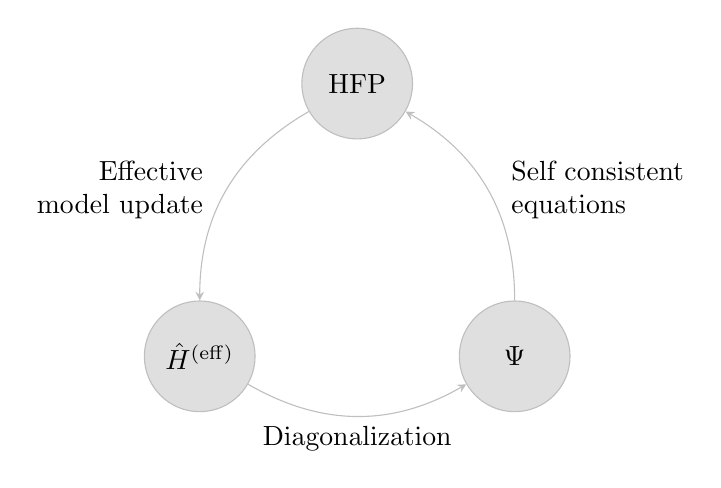
\begin{tikzpicture} 
	
    \node[
        name=he,
        circle,
        draw=lightgray,
        text=black,
        fill=lightgray!50,
        minimum size=4em
    ] 
        (He) at (0,0)
            {$\hat H^{(\mathrm{eff})}$};
            
    \node[
        name=psi,
        circle,
        draw=lightgray,
        text=black,
        fill=lightgray!50,
        minimum size=4em
    ] 
        (PSI) at (4,0)
            {$\ket{\Psi}$};
            
    \node[
        name=hfp,
        circle,
        draw=lightgray,
        text=black,
        fill=lightgray!50,
        align=center,
        minimum size=4em
    ] 
        (HFP) at (2,3.464)
            {HFP};
            
    \draw[color=lightgray, -stealth]
        (He) to[bend right]node[below,color=black]{Diagonalization} (PSI);
    \draw[color=lightgray, -stealth]
        (PSI) to[bend right]node[right,color=black,align=left,xshift=0.5em]{Self consistent\\equations} (HFP);
    \draw[color=lightgray, -stealth]
        (HFP) to[bend right]node[left,color=black,align=right,xshift=-0.5em]{Effective\\model update} (He);

\end{tikzpicture}

	\caption{Schematization of the self-consistent Hartree Fock method described in Sec.~\ref{sec:computational-mft}. The effective model is solved, the solution is used to estimate self-consistently the Hartree Fock vector, which is then used to update iteratively the model itself.}
	\label{fig:effective-model-scheme}
\end{figure}
%
A self consistent Hartree-Fock scheme goes as follows: {\color{tabred}[ Consider adding a point for chemical potential estimation. ]}
\begin{enumerate}
	\item Apply MFT to the quartic hamiltonian, recovering its general theoretic effective form;
	\item Impose selection rules on the parameters $C_{\alpha\beta}$, $D_{\alpha\beta}$, eventually eliminating those not respecting the symmetry sector we are working in\footnote{
		As an example: if we choose not to break charge conservation, set $\forall\alpha,\beta\,\colon\,D_{\alpha\beta}=0$.
	};
	\item Choose a starting value and a coherent symmetry structure for the remaining parameters;
	\item Enter iterative scheme of Fig.~\ref{fig:effective-model-scheme}:
	\begin{enumerate}
		\item Diagonalize the effective hamiltonian $\hat H^{(\mathrm{eff})}[C,D]$ and recover the ground-state $\ket{\Psi [C,D]}$;
		\item Compute the new parameters $C_{\alpha\beta}'$, $D_{\alpha\beta}'$ via the self consistent equations;
		\item Initialize the new effective hamiltonian $\hat H^{(\mathrm{eff})}[C',D']$ and repeat the cycle until convergence.
	\end{enumerate}
\end{enumerate}
Of course, to work any of these algorithms we need to know how to diagonalize the hamiltonian. In the context of the Extended Hubbad Model at thermal equilibrium, due to the phases we are simulating, we know analytically the diagonalized hamiltonian, and making use of this knowledge we are able to reduce the self consistent scheme to a simple iterative algorithm. An explicit example of HF algorithm used in present text, somewhat simplified due to the presence of a single HF parameter, is given in App.~\ref{appsubsec:hartree-fock-algorithm}.

\subsection{Square lattice spatial symmetry structures}

\begin{figure}
	\centering
	\subfloat[Local $s$-wave]{
		\begin{tikzpicture}
	\fill[color=lightgray] 
	(0,0) circle (1.5pt)
		node[anchor=south west, color=black]
			{$1$}
	(1,0) circle (1.5pt)
		node[anchor=west]
			{$0$}
	(-1,0) circle (1.5pt)
		node[anchor=east]
			{$0$}
	(0,1) circle (1.5pt)
		node[anchor=south]
			{$0$}
	(0,-1) circle (1.5pt)
		node[anchor=north]
			{$0$};
			
	\node[anchor=center] 
		at (-1,1)
			{$\varphi^{(s)}_{ij}$};
	
	\draw[color=lightgray, dashed]
		(-1,0) -- (1,0)
		(0,-1) -- (0,1);
\end{tikzpicture}
		\label{subfig:s-wave-correlator}
	}
	\hspace{2em}
	\subfloat[Extended $s$-wave.]{
		\begin{tikzpicture}
	\fill[color=lightgray] 
	(0,0) circle (1.5pt)
	(1,0) circle (1.5pt)
		node[anchor=west, color=black]
			{$g^{(s)}$}
	(-1,0) circle (1.5pt)
		node[anchor=east, color=black]
			{$g^{(s)}$}
	(0,1) circle (1.5pt)
		node[anchor=south, color=black]
			{$g^{(s)}$}
	(0,-1) circle (1.5pt)
		node[anchor=north, color=black]
			{$g^{(s)}$};
	
	\draw[color=lightgray]
	(-1,0) -- (1,0)
	(0,-1) -- (0,1);
\end{tikzpicture}
		\label{subfig:s*-wave-correlator}
	}\\[3em]
	\subfloat[$p_x$-wave.]{
		\begin{tikzpicture}
	\fill[color=lightgray] 
	(0,0) circle (1.5pt)
		node[anchor=south west]
			{$0$}
	(1,0) circle (1.5pt)
		node[anchor=west, color=black]
			{$1$}
	(-1,0) circle (1.5pt)
		node[anchor=east, color=black]
			{$-1$}
	(0,1) circle (1.5pt)
		node[anchor=south]
			{$0$}
	(0,-1) circle (1.5pt)
		node[anchor=north]
			{$0$}
	(0,-1) circle (1.5pt)
		node[anchor=north, opacity=0]
			{$-1$}; % Aligment
			
	\node[anchor=center] 
		at (-1,1)
			{$\varphi^{(p_x)}_{ij}$};
	
	\draw[color=lightgray] 
		(-1,0) -- (1,0);
	\draw[color=lightgray, dashed] 
		(0,-1) -- (0,1);
\end{tikzpicture}
		\label{subfig:px-wave-correlator}
	}
	\hspace{2em}
	\subfloat[$p_y$-wave.]{
		\begin{tikzpicture}
	\fill[color=lightgray] 
	(0,0) circle (1.5pt)
	(1,0) circle (1.5pt)
		node[anchor=west, color=black]
			{$0$}
	(-1,0) circle (1.5pt)
		node[anchor=east, color=black]
			{$0$}
	(0,1) circle (1.5pt)
		node[anchor=south, color=black]
			{$g^{(p_y)}$}
		node[anchor=south, opacity=0] 
			{$g^{(d_{x^2-y^2})}$} 	% Alignment
	(0,-1) circle (1.5pt)
		node[anchor=north, color=black]
			{$-g^{(p_y)}$}
		node[anchor=north, opacity=0] 
			{$g^{(d_{x^2-y^2})}$};	% Alignment;
	
	\draw[color=lightgray, dashed] 
		(-1,0) -- (1,0);
	\draw[color=lightgray] 
		(0,-1) -- (0,1);
\end{tikzpicture}
		\label{subfig:py-wave-correlator}
	}
	\hspace{2em}
	\subfloat[$d_{x^2-y^2}$-wave.]{
		\begin{tikzpicture}
	\fill[color=lightgray] 
	(0,0) circle (1.5pt)
	(1,0) circle (1.5pt)
		node[anchor=west, color=black]
			{$g^{(d_{x^2-y^2})}$}
	(-1,0) circle (1.5pt)
		node[anchor=east, color=black]
			{$g^{(d_{x^2-y^2})}$}
	(0,1) circle (1.5pt)
		node[anchor=south, color=black]
			{$-g^{(d_{x^2-y^2})}$}
	(0,-1) circle (1.5pt)
		node[anchor=north, color=black]
			{$-g^{(d_{x^2-y^2})}$};
	
	\draw[color=lightgray] 
		(-1,0) -- (1,0)
		(0,-1) -- (0,1);
\end{tikzpicture}
		\label{subfig:d-wave-correlator}
	}
	\caption{Form factors at different topologies, as listed in Tab.~\ref{tab:x-wave-real-factors}. In figures five sites are represented: the hub site $i$ and its four NN. Solid lines represent non-zero values for $\varphi_{\bm{\delta}}$, while dashed lines represent vanishing factors.}
	\label{fig:x-wave-real-factors}
\end{figure}

For the $2$D square lattice, various spatial symmetries are possible. Let $i$ be a specific site, and consider a generic function $g_{ij}$ whose domain is given by the site itself and its four NNs (the domain concides with the points of Fig.~\ref{fig:square-nearest-neighbors}). Then it is immediate to see that the function can be written in the following basis
\[
	g_{ij} = \sum_\gamma g^{(\gamma)} \varphi_{ij}^{(\gamma)}
\]
where $g^{(\gamma)}$ are the $g_{ij}$ symmetries-decomposition coefficients while $\varphi_{ij}^{(\gamma)}$ are the form factors listed in Tab.~\ref{tab:x-wave-real-factors}, a simple orthonormal rearrangement of the harmonics basis.

\setlength{\extrarowheight}{0.5em}
\begin{table}
	\centering
	\begin{tabular}{r E l l}
		\textbf{Structure} & \multicolumn{2}{c}{\textbf{Form factor}} & \textbf{Graph} \\
		\midrule
		$s$-wave & $\varphi^{(s)}_{ij}$ & $\delta_{ij}$ & Fig.~\ref{subfig:s-wave-correlator} \\
		Extended $s$-wave & $\varphi^{(s^*)}_{ij}$ &
		$\delta_{j=i+\delta_x} + \delta_{j=i-\delta_x} + \delta_{j=i+\delta_y} + \delta_{j=i-\delta_y}$ & Fig.~\ref{subfig:s*-wave-correlator} \\
		$p_x$-wave & $\varphi^{(p_x)}_{ij}$ & $ 
		\delta_{j=i+\delta_x} - \delta_{j=i-\delta_x}$ & Fig.~\ref{subfig:px-wave-correlator} \\
		$p_y$-wave & $\varphi^{(p_y)}_{ij}$ & $ \delta_{j=i+\delta_y} - \delta_{j=i-\delta_y}$ & Fig.~\ref{subfig:py-wave-correlator} \\
		$d_{x^2-y^2}$-wave & $\varphi^{(d)}_{ij}$ & $
		\delta_{j=i+\delta_x} + \delta_{j=i-\delta_x} - \delta_{j=i+\delta_y} - \delta_{j=i-\delta_y}$ & Fig.~\ref{subfig:d-wave-correlator} \\[0.5em]
		\midrule
	\end{tabular}
	\caption{Form factors for a function defined on a square lattice,- The last column indicates the graph representation of each contribution given in Fig.~\ref{fig:wave-correlators}. Subscript $x^2-y^2$ is omitted for notational clarity.}
	\label{tab:x-wave-real-factors}
\end{table}
\setlength{\extrarowheight}{0em}

Antiferromagnetic ordering considered in this text exhibits a perfect $s \oplus s^*$ topological ordering. Instead, superconductivity is established with a given symmetry -- which means, symmetry breaking in the phase transition proceeds in a specific channel. Conventional $\mathrm{BCS}$ superconductivity arises from the only possible spatial structure of the local pairing, $s$-wave -- here appearing as a local term (Fig.~\ref{subfig:s-wave-correlator}) and extended on a non-local term (Fig.~\ref{subfig:s*-wave-correlator}). Cuprates exhibit a tendency towards $d_{x^2-y^2}$ SC, while other materials towards $p$-wave types -- eventually with some chirality, as is the case for $p_x \pm i p_y$ SCs. To establish SC under a certain symmetry $\gamma$ means that Cooper pairs acquire said symmetry.

\subsection{Symmetry-based optimizations}

When dealing with phases which respect translational symmetry, or at most reduce it to a weaker symmetry by shrinking the Brillouin Zone, it' useful to work in reciprocal space, as discussed in Sec.~\ref{sec:mft-analysis-reciprocal-space}. As said, a particular phase can show specific spatial symmetries, and so will the Hartree Fock parameters. The key point to notice is that self-consistent equations involve sums (or integrals) to be computed over fermionic states, which can be heavily simplified by employing said symmetries. Consider the form factors of Tab.~\ref{tab:x-wave-real-factors}, and their Fourier transforms of Tab.~\ref{tab:x-wave-reciprocal-factors}. If these symmetries are developed by the HFPs, it's of no use to integrate over the entire BZ, since different regions linked by periodicity of the form factors will lead to redundant calculations.

{\color{tabred}[
	Add: plots of the Brillouin zone cut for different symmetries.
]}

\setlength{\extrarowheight}{0.5em}
\begin{table}
	\centering
	\begin{tabular}{r E l l}
		\textbf{Structure} & \multicolumn{2}{c}{\textbf{Structure factor}} & \textbf{Graph} \\
		\midrule
		$s$-wave & $\varphi_\mathbf{k}^{(s)}$ & $1$ & Fig.~\ref{subfig:s-wave-correlator} \\
		Extended $s$-wave & $\varphi^{(s^*)}_{\mathbf{k}}$ & $\cos k_x + \cos k_y$ & Fig.~\ref{subfig:s*-wave-correlator} \\
		$p_x$-wave & $\varphi_\mathbf{k}^{(p_x)}$ & $i \sqrt{2} \sin k_x $ & Fig.~\ref{subfig:px-wave-correlator} \\
		$p_y$-wave & $\varphi_\mathbf{k}^{(p_y)}$ & $i \sqrt{2} \sin k_y$ & Fig.~\ref{subfig:py-wave-correlator} \\
		$d_{x^2-y^2}$-wave & $\varphi_\mathbf{k}^{(d)}$ & $\cos k_x - \cos k_y$ & Fig.~\ref{subfig:d-wave-correlator} \\[0.5em]
		\midrule
	\end{tabular}
	\caption{Structure factors derived from the correlation structures of Tab.~\ref{tab:x-wave-real-factors}. The functions hereby defined are orthonormal.}
	\label{tab:x-wave-reciprocal-factors}
\end{table}
\setlength{\extrarowheight}{0em}

Finally, a very useful detail is given by the following argument. Consider the equation
\[
	\cos \left( \delta k_x \right)	+ \cos \left( \delta k_y \right) = \cos k_x \cos k_x' + \sin k_x \sin k_x' + \cos k_y \cos k_y' + \sin k_y \sin k_y'
\]
For the sake of readability, the notations
\[
	c_\ell \equiv \cos k_\ell
	\qquad
	s_\ell \equiv \sin k_\ell
	\qquad
	c_\ell' \equiv \cos	k_\ell'
	\qquad
	s_\ell' \equiv \sin k_\ell'
\]
are used. Group the four terms above,
\begin{equation}\label{eq:sym-asym-couplings-gap}
	\underbrace{
		\left(c_x c_x' + c_y c_y' \right) 
	}_\text{Symmetric}
	+ \underbrace{
		\left(s_x s_x' + s_y s_y' \right)
	}_\text{Anti-symmetric}
\end{equation}
The first two exhibit inversion symmetry for both arguments $\mathbf{k}$, $\mathbf{k}'$; the second two exhibit anti-symmetry. Decoupling the symmetric part, we obtain
\[
	c_x c_x' + c_y c_y' = \frac{1}{2} (c_x + c_y)(c_x' + c_y') + \frac{1}{2} (c_x - c_y)(c_x' - c_y')
\]
which finally gives:
\[
\begin{aligned}
	\cos \left( \delta k_x \right)	+ \cos \left( \delta k_y  \right) &= \frac{1}{2}  (c_x + c_y)(c_x' + c_y') &&\qquad\text{($s^*$-wave)} \\
	&\hphantom{=}+ s_x s_x' &&\qquad\text{($p_x$-wave)} \\
	&\hphantom{=}+ s_y s_y' &&\qquad\text{($p_y$-wave)} \\
	&\hphantom{=}+ \frac{1}{2} (c_x - c_y)(c_x' - c_y') &&\qquad\text{($d_{x^2-y^2}$-wave)}
\end{aligned}
\]
or, in a more compact form	
\begin{equation}\label{eq:coscos-symmetries-decomposition}
	\cos \left( \delta k_x \right)	+ \cos \left( \delta k_y  \right) = \frac 1 2 \sum_\gamma \varphi_\mathbf{k}^{(\gamma)} \varphi_{\mathbf{k}'}^{(\gamma)*}
	\qq{for $\gamma \in \lbrace s^*, p_x, p_y, d_{x^2-y^2} \rbrace$}
\end{equation}
This decomposition will become particularly handy in later calculations.